\begin{frame}[c]\label{b.1}
\frametitle{A Theory of Localized Excitations: Pure Shear Excitations}

\vspace{-0.5em}
\begin{block}{\centering \large Origin of Excitations }
\centering The inherent \textbf{structure and elasticity (solid-like)} of supercooled liquids $\leftrightarrow$ localized excitations! {\footnotesize (Hasyim, Mandadapu,  \textit{J. Chem. Phys.} 155, 044504 2021)}
\end{block}
\vspace{-0.5em}
\begin{columns}[T]
\begin{column}[T]{0.4\textwidth}

\begin{figure}[t]

\begin{overprint}
\onslide<2>\centering\includegraphics[width=1.1\linewidth]{5.c-fac_summodel/PEL.pdf}\caption{Glassy dynamics is hopping between energy minima (inherent states)  (Stillinger and Weber, \textit{Phys. Rev. A} 1982)}

\onslide<3>\centering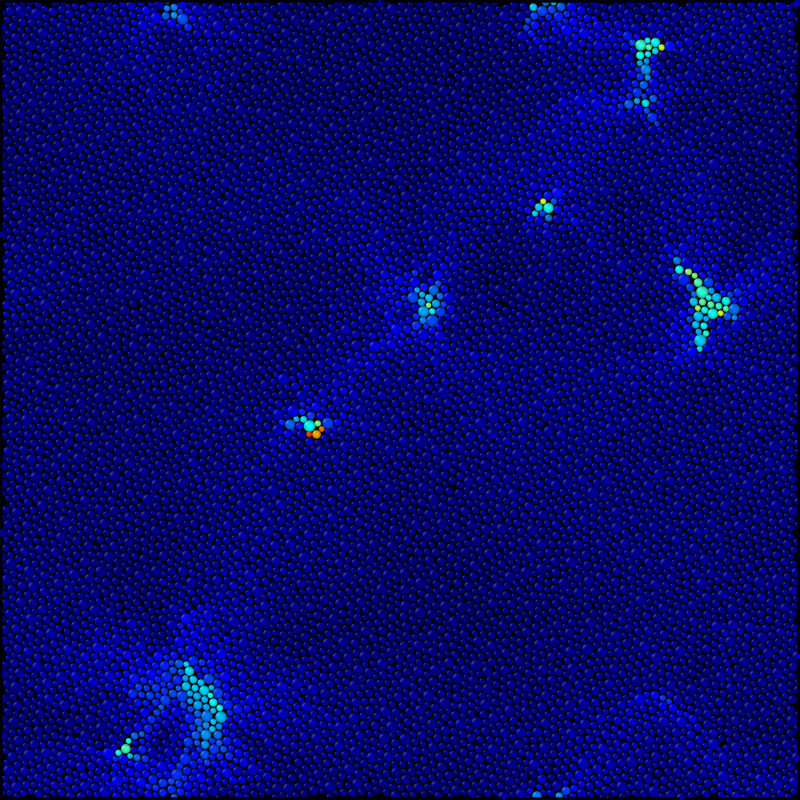
\includegraphics[width=0.85\linewidth]{1.b-exc_pureshear/zoomout_dispmag.png}\caption{Excitations of a model glass former, detected by the initial dynamic heterogeneity.}

\onslide<4>\centering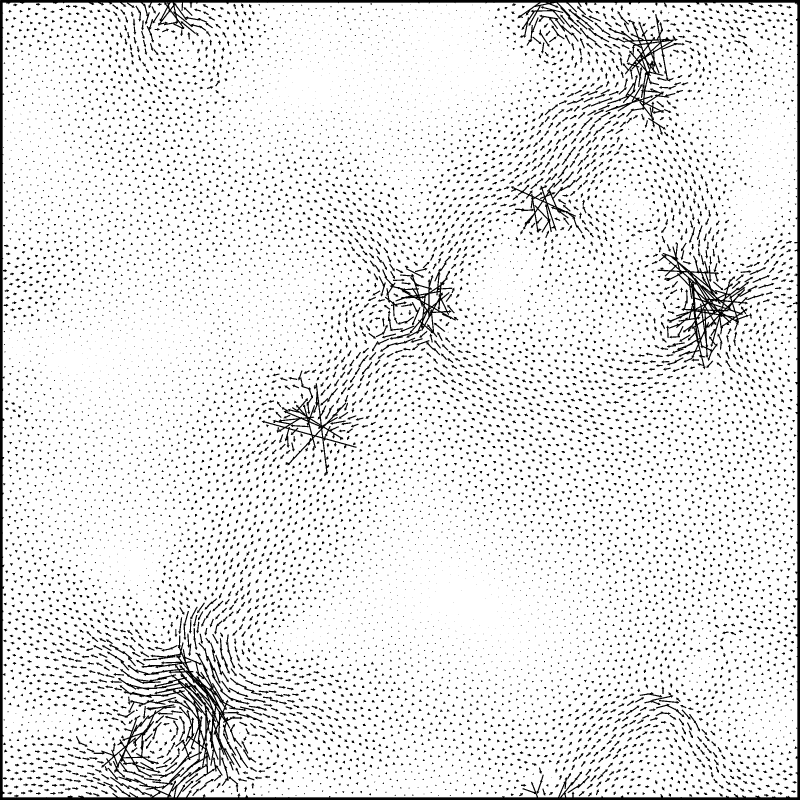
\includegraphics[width=0.85\linewidth]{1.b-exc_pureshear/zoomout_dispvector.png}\caption{The displacement vector field due to excitations in the liquid.}

\onslide<5>\centering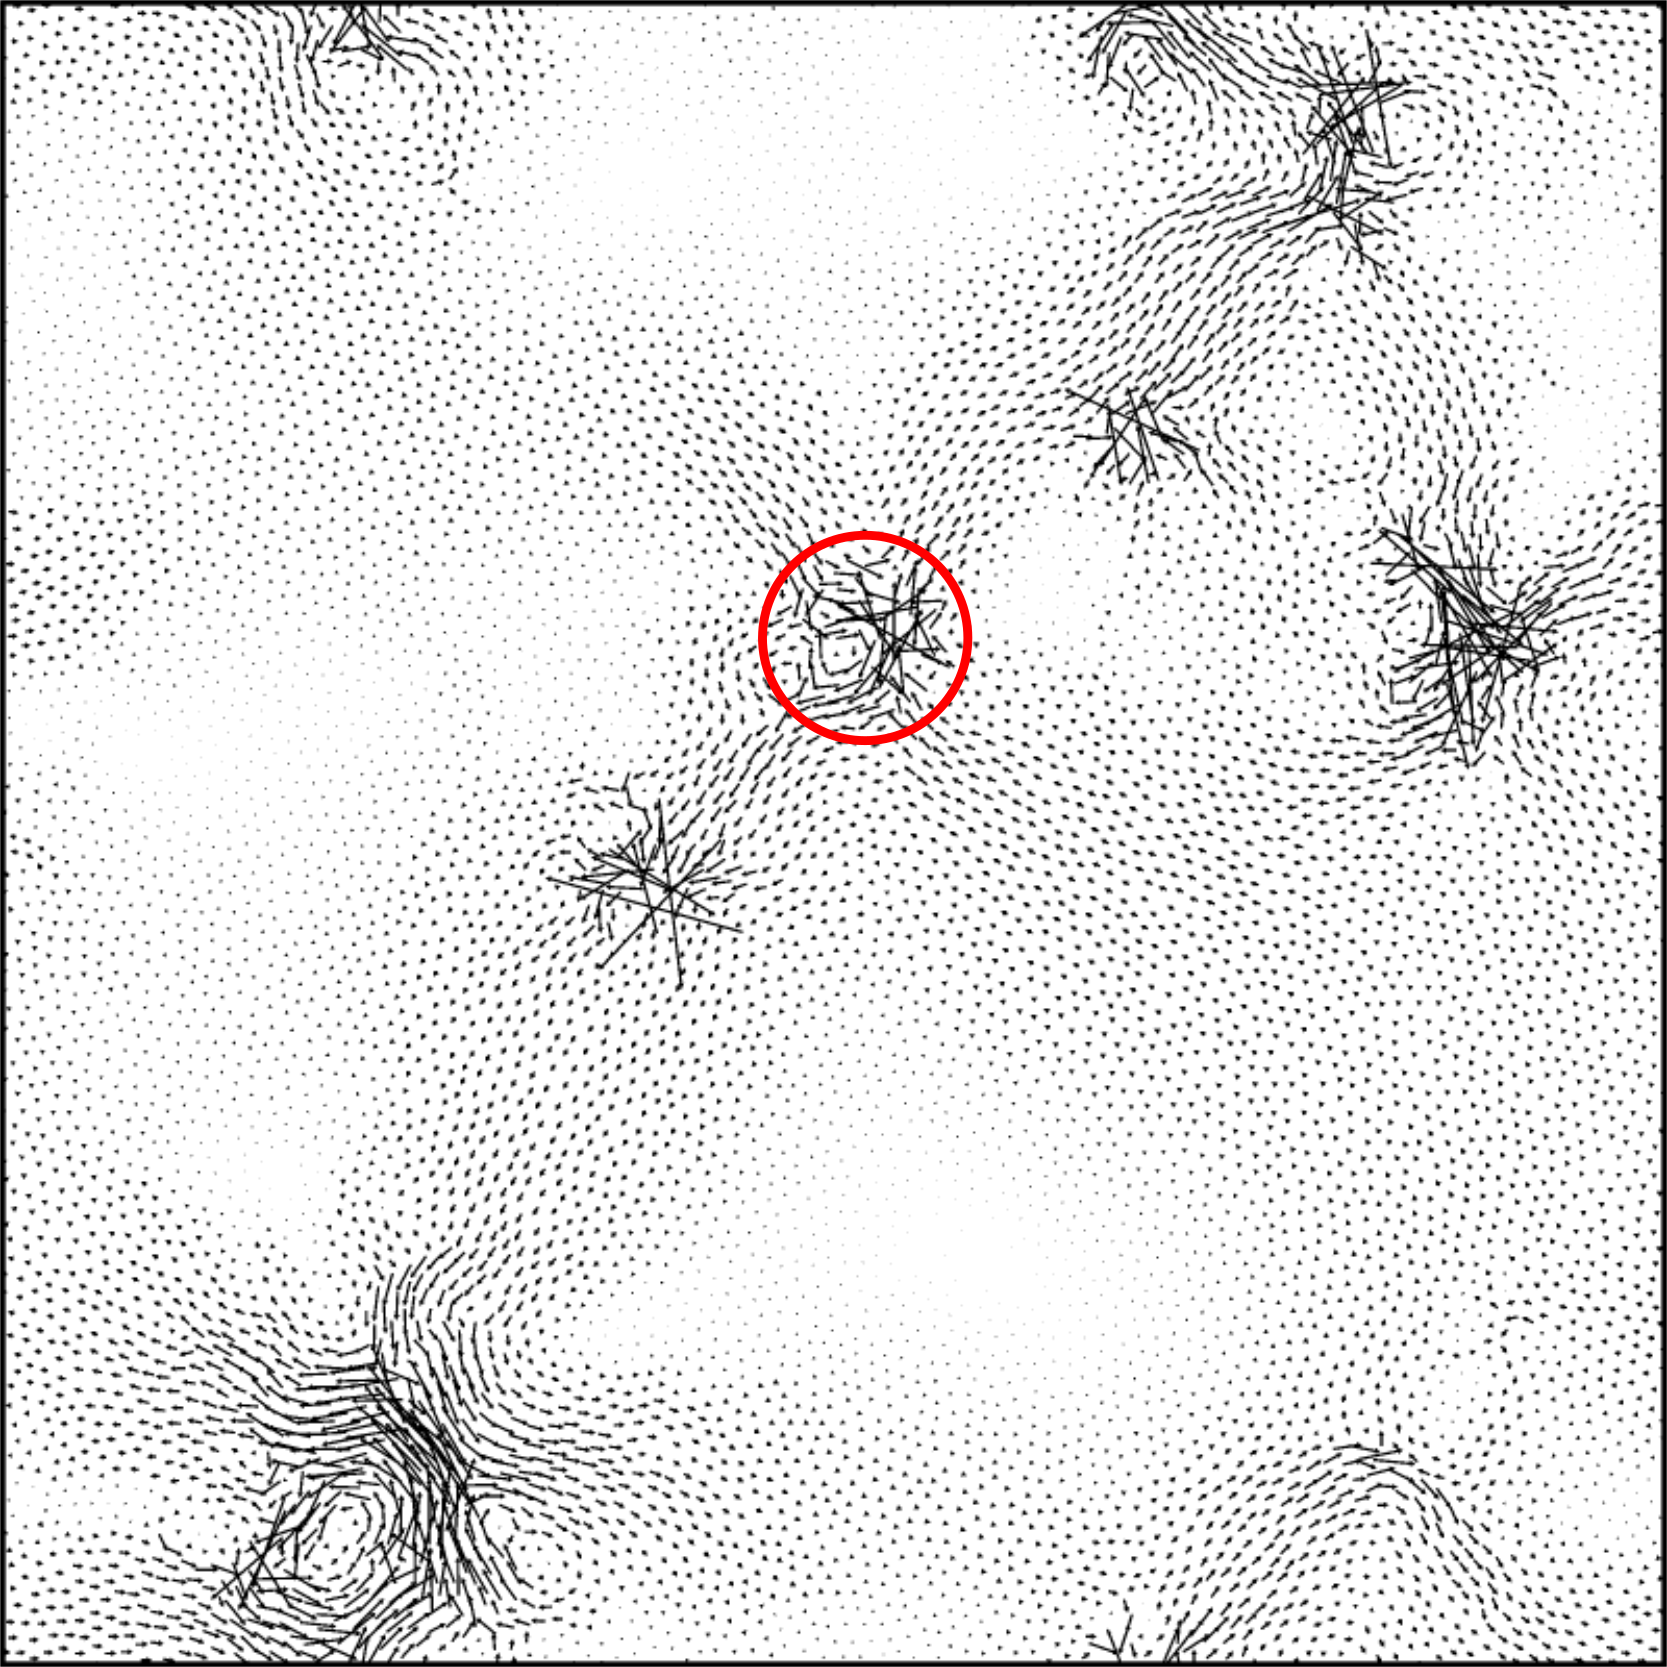
\includegraphics[width=0.85\linewidth]{1.b-exc_pureshear/zoomout_dispvector_1.png}\caption{The displacement field vector field due to excitations in the liquid.}

\onslide<6>\centering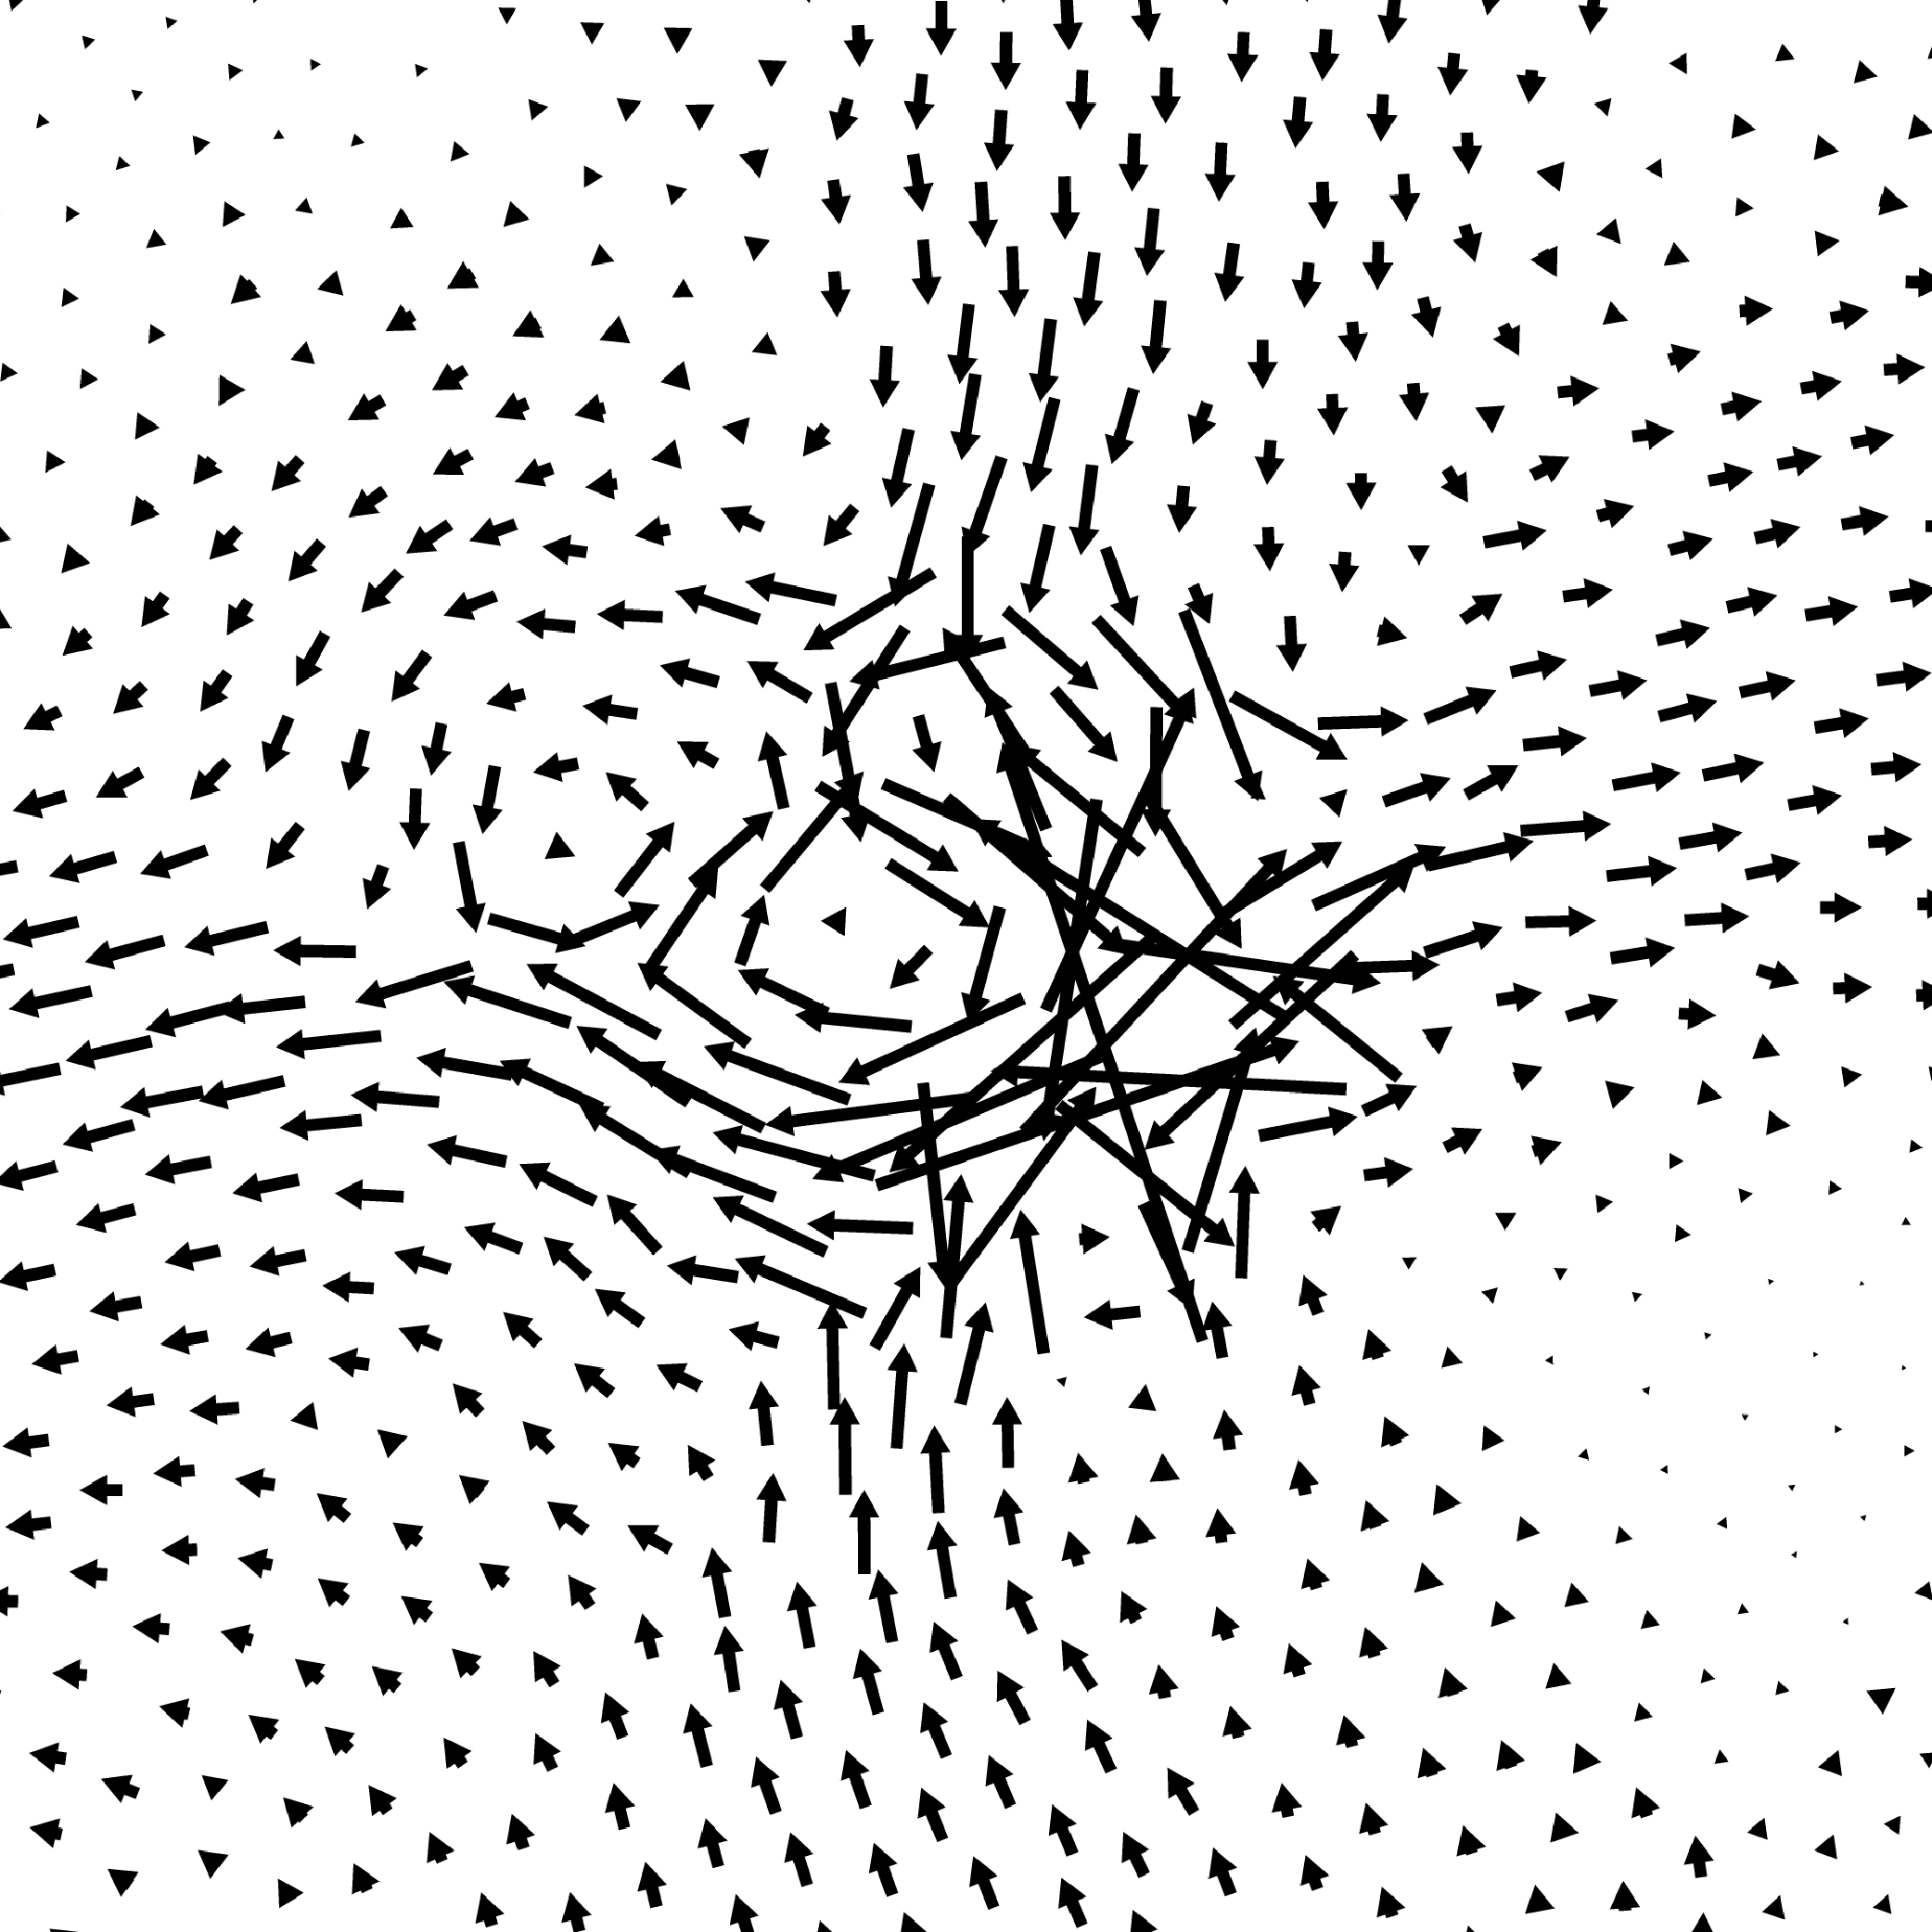
\includegraphics[width=0.85\linewidth]{1.b-exc_pureshear/zoomin-0.pdf}\caption{An excitation reorganizes the surrounding solid medium.}

\onslide<7>\centering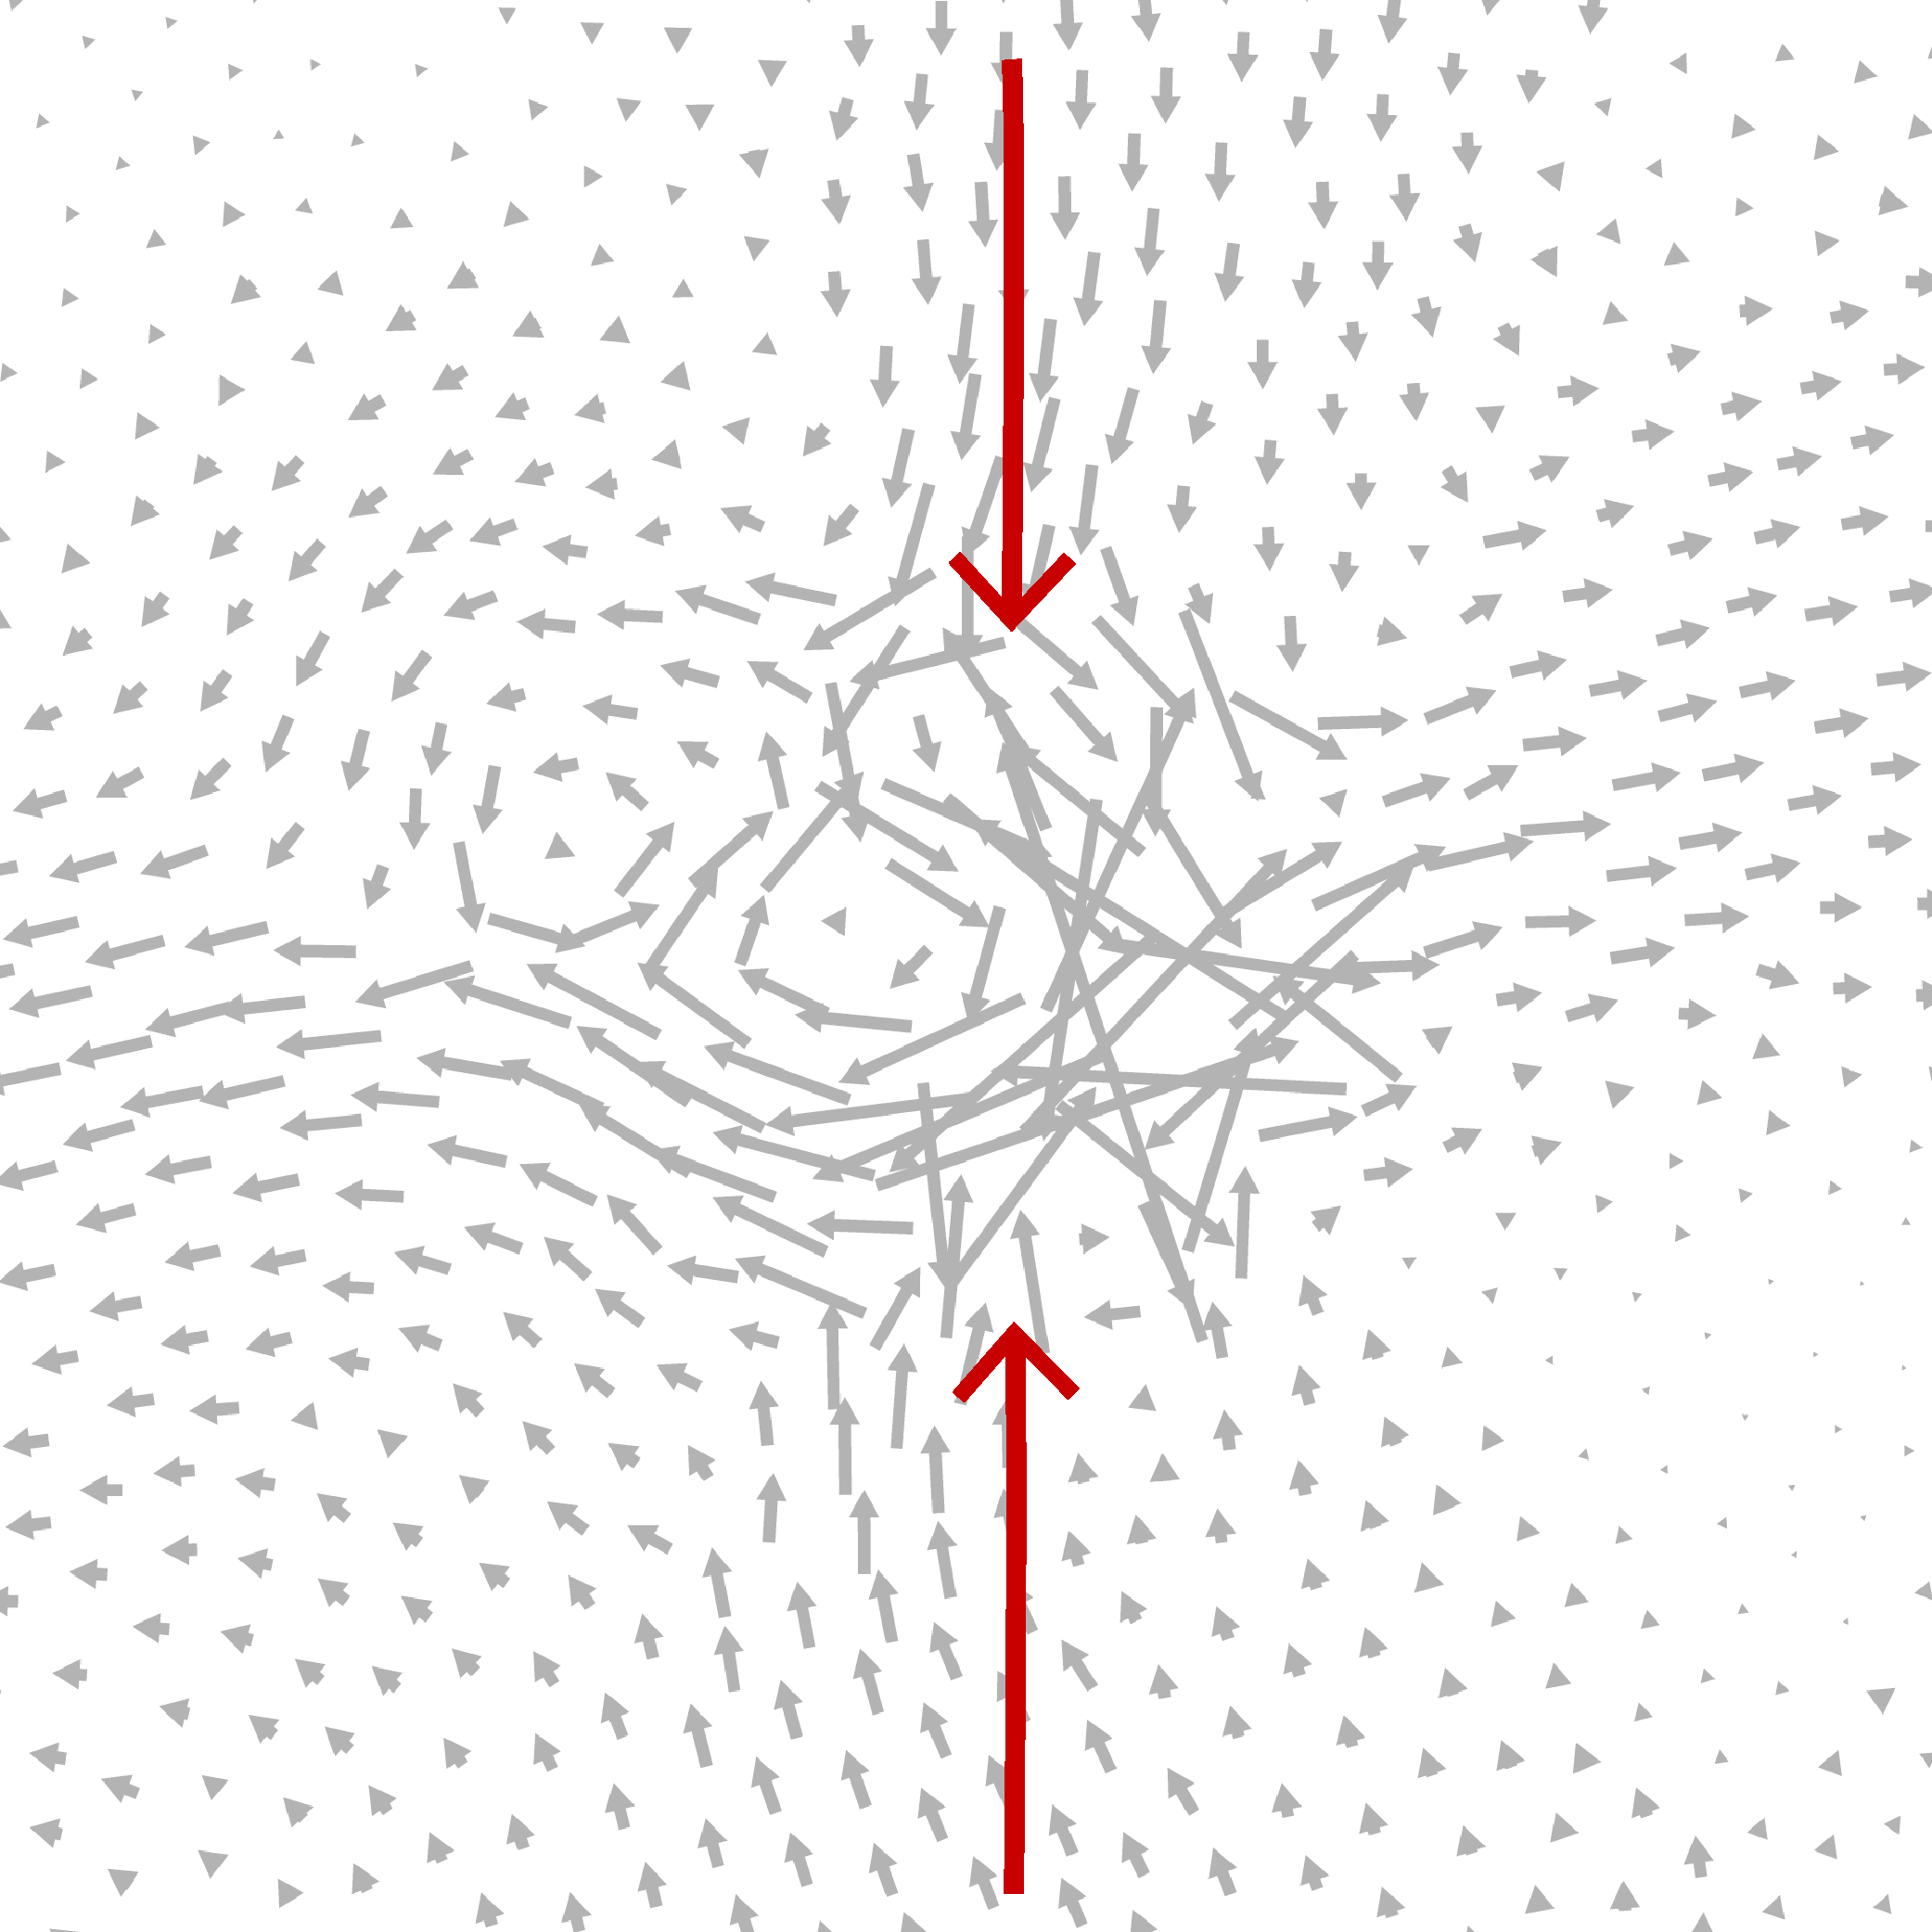
\includegraphics[width=0.85\linewidth]{1.b-exc_pureshear/zoomin-1.pdf}\caption{In one axis, there's compressive flow.}

\onslide<8>\centering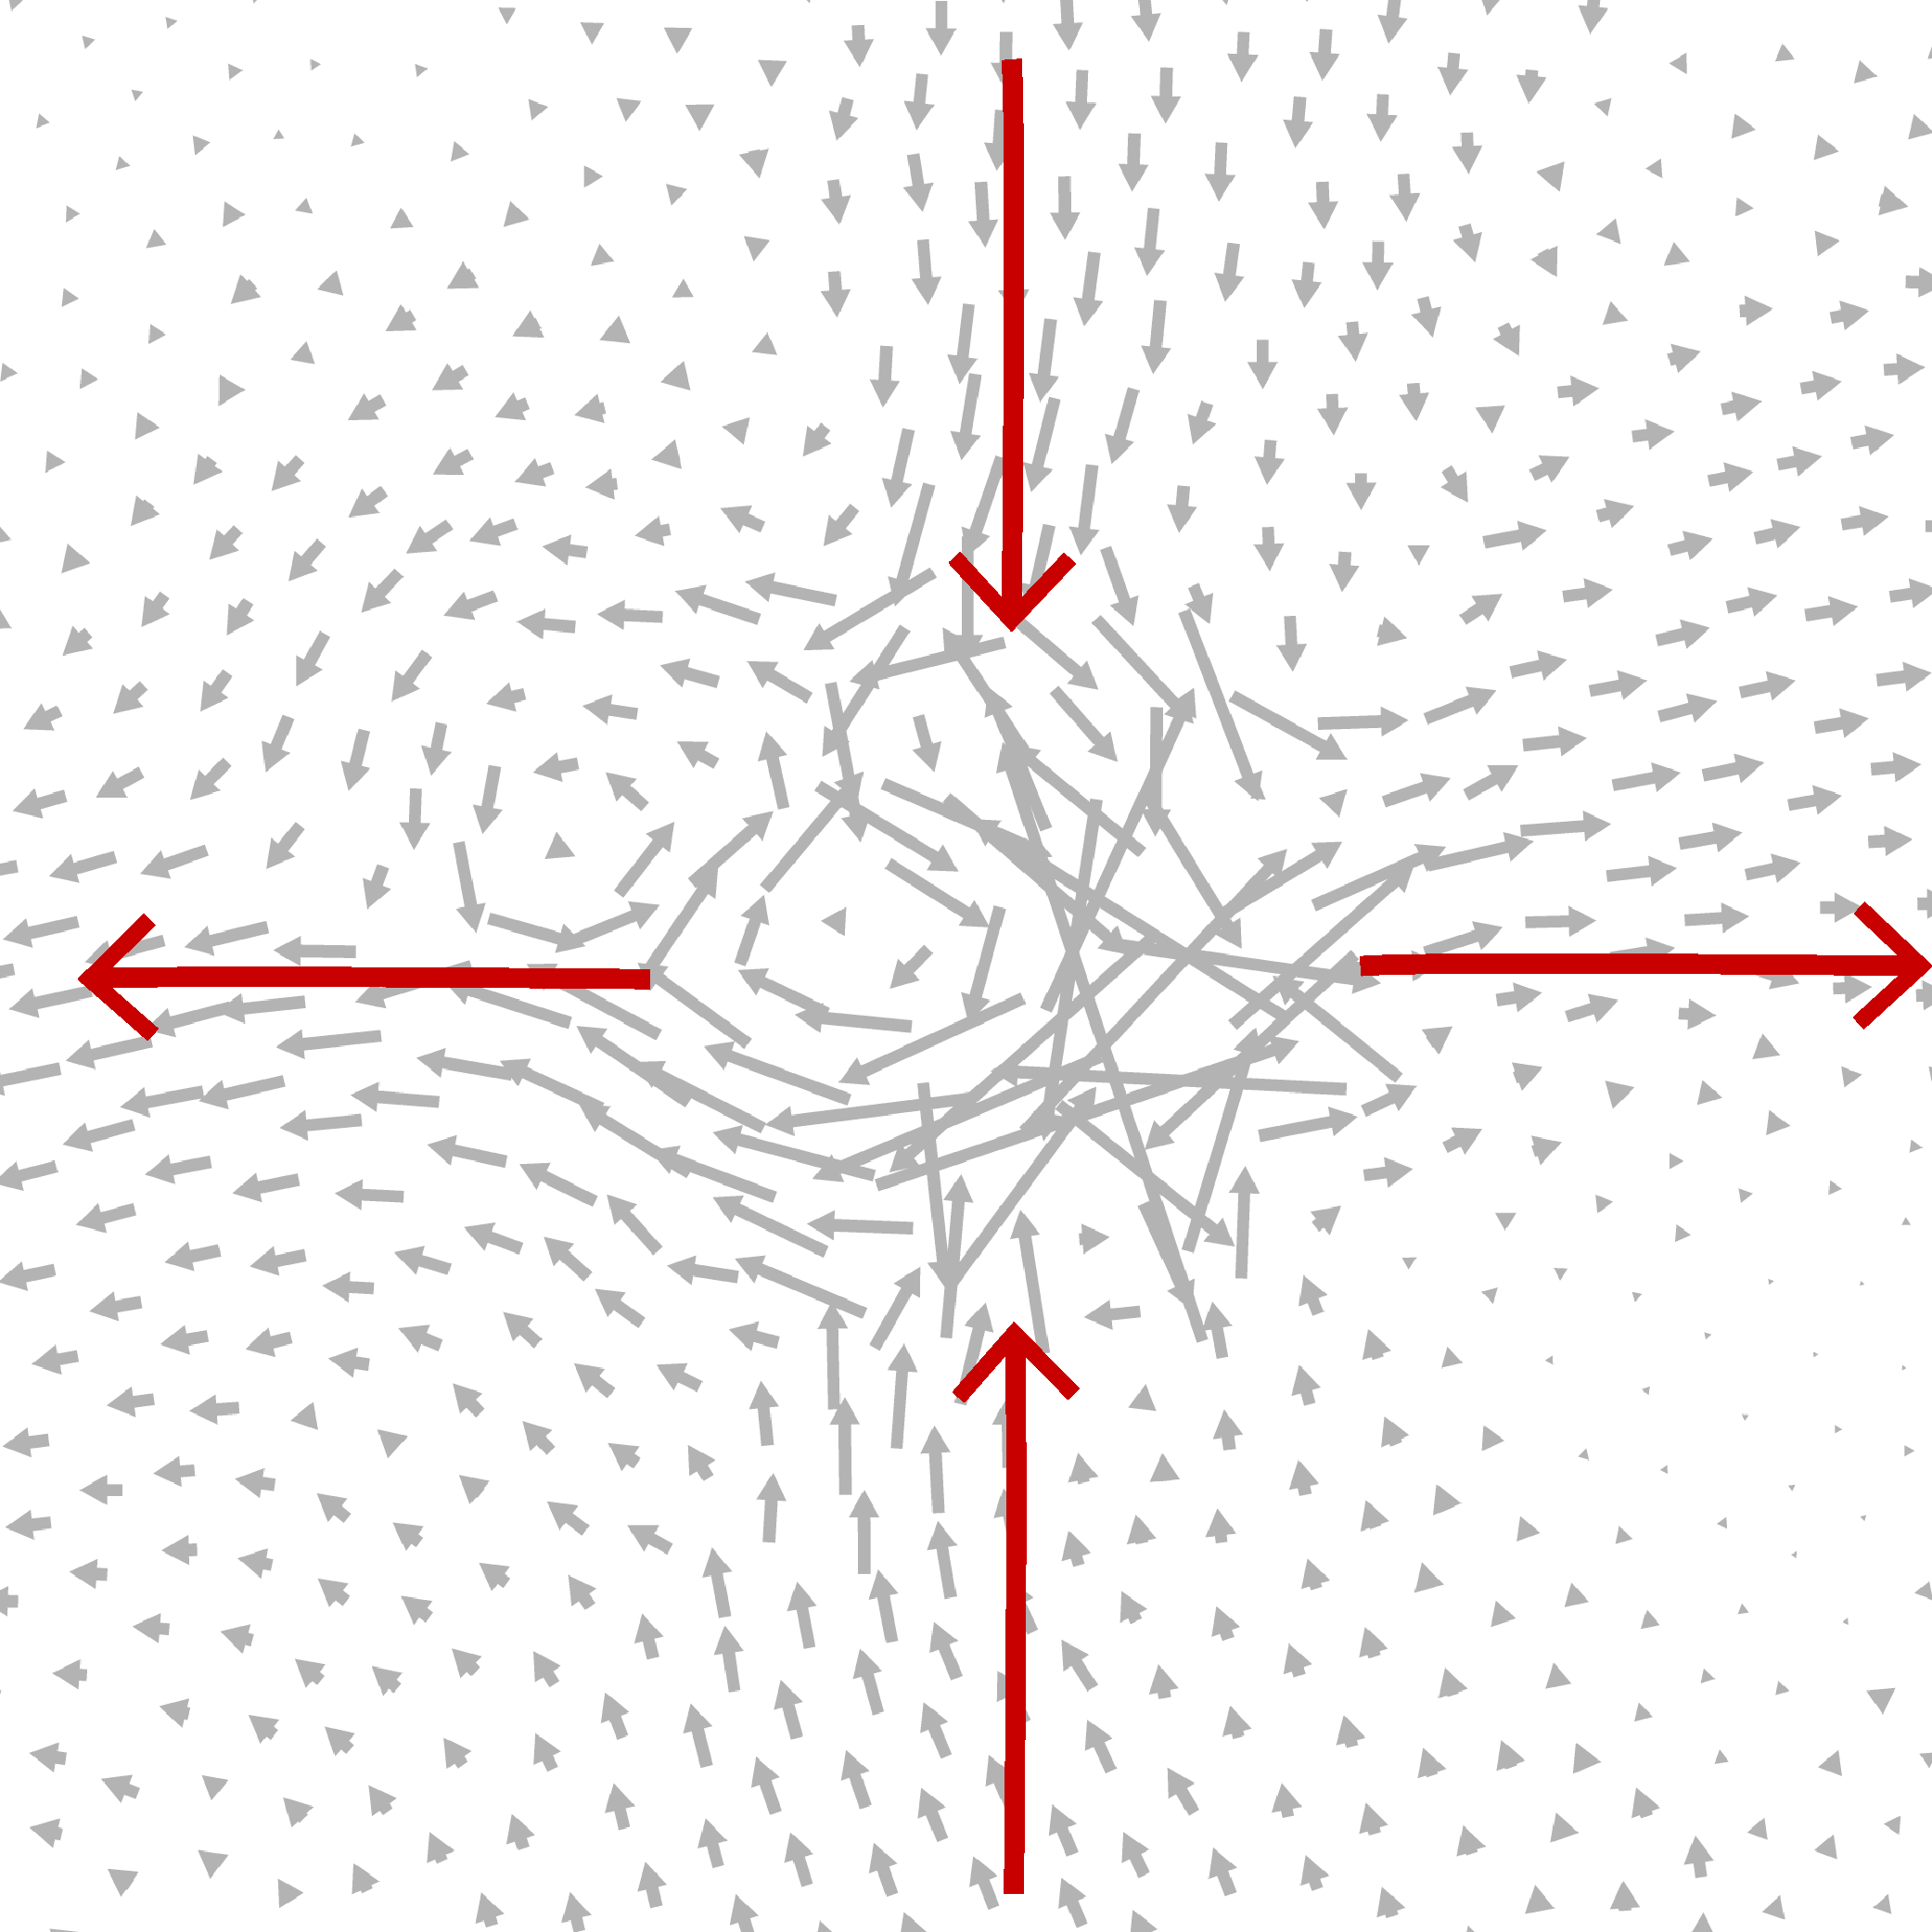
\includegraphics[width=0.85\linewidth]{1.b-exc_pureshear/zoomin-2.pdf}\caption{In another axis, there's extensile flow.}

\onslide<9>\centering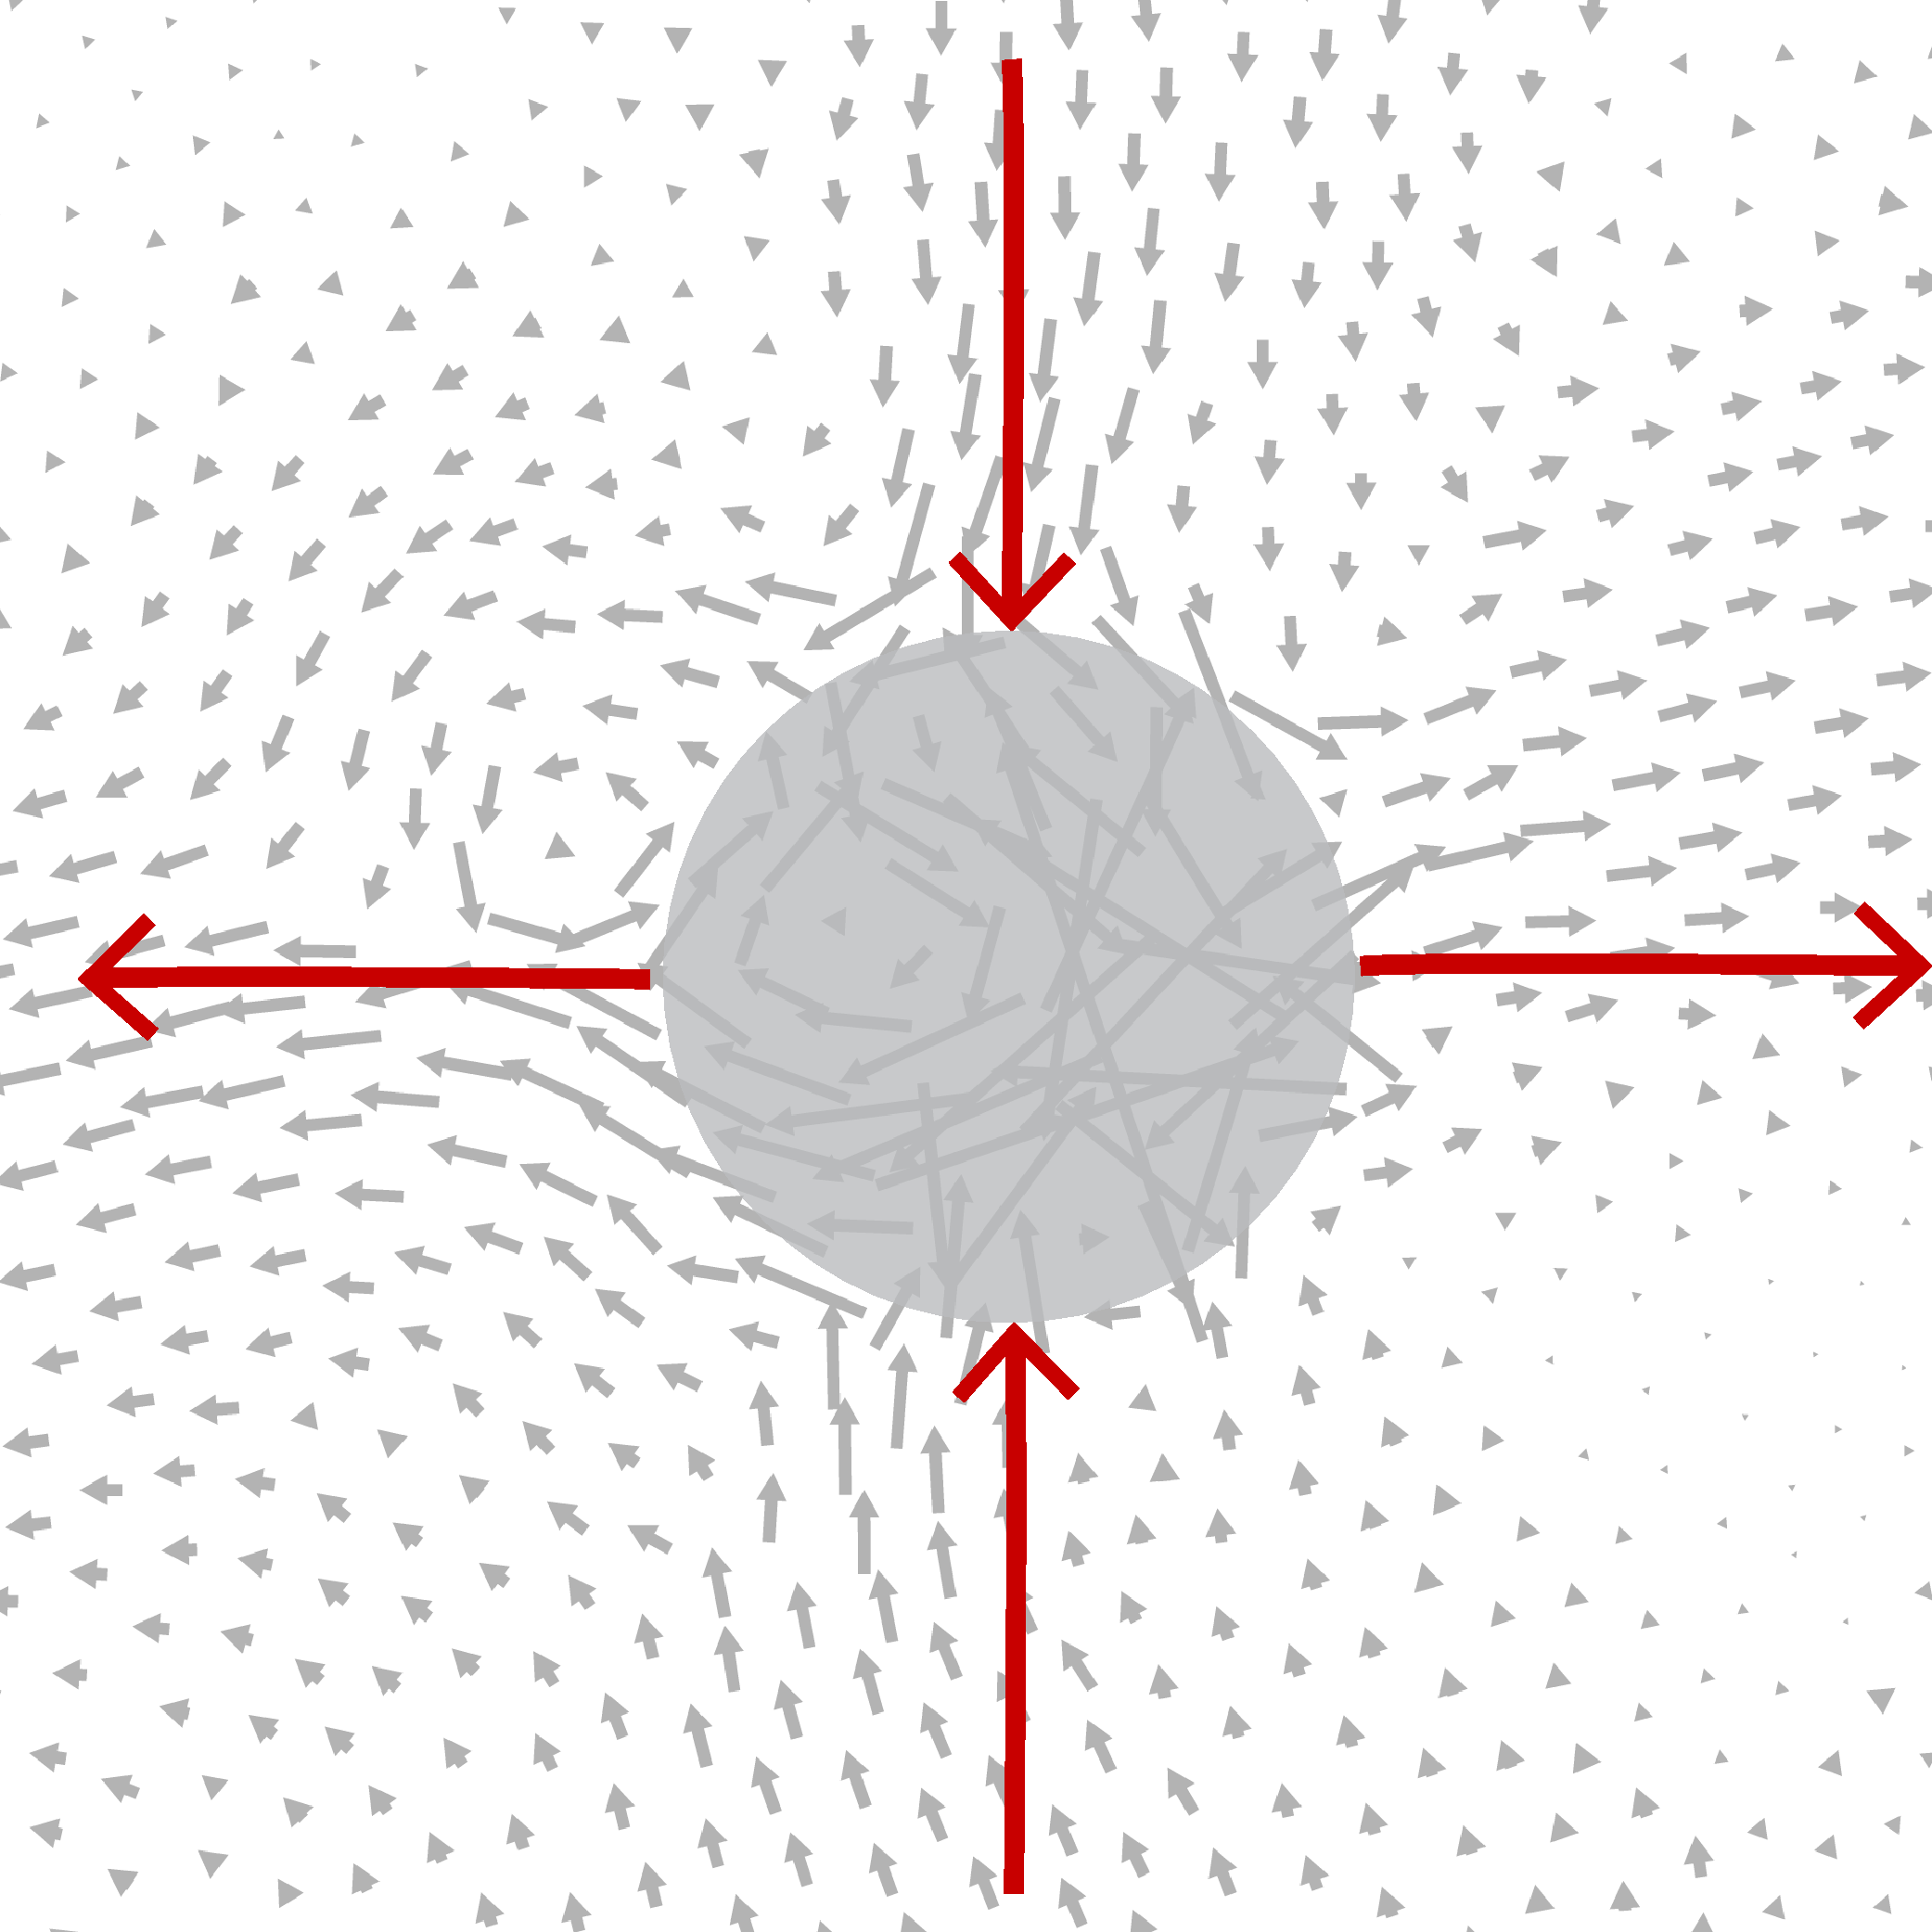
\includegraphics[width=0.85\linewidth]{1.b-exc_pureshear/zoomin-3.pdf}\caption{Compressive + extensile flow = \textbf{a pure shear deformation} {\footnotesize (Lemaitre, \textit{PRL} 2014).}}

\onslide<10>\centering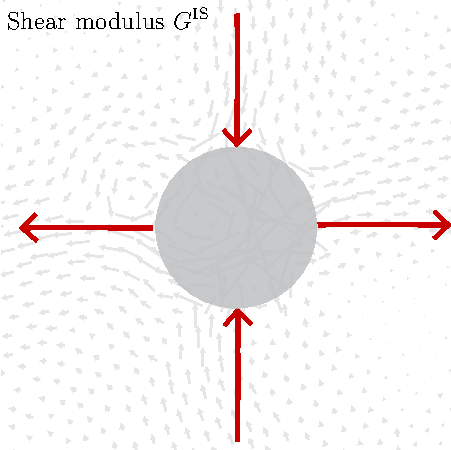
\includegraphics[width=0.85\linewidth]{1.b-exc_pureshear/zoomin-7.pdf}\caption{Compressive + extensile flow = \textbf{a pure shear deformation} {\footnotesize (Lemaitre, \textit{PRL} 2014).}}

\onslide<11>\centering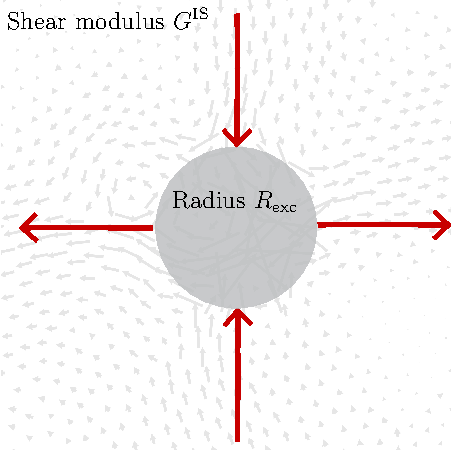
\includegraphics[width=0.85\linewidth]{1.b-exc_pureshear/zoomin-8.pdf}\caption{Compressive + extensile flow = \textbf{a pure shear deformation} {\footnotesize (Lemaitre, \textit{PRL} 2014).}}

\onslide<12-14>\centering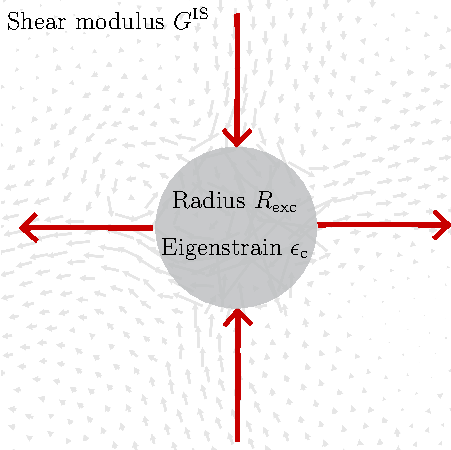
\includegraphics[width=0.85\linewidth]{1.b-exc_pureshear/zoomin-9.pdf}\caption{Compressive + extensile flow = \textbf{a pure shear deformation} (Lemaitre, \textit{PRL} 2014).}

\onslide<15->\centering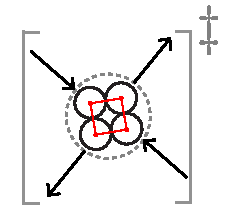
\includegraphics[width=0.85\linewidth]{1.b-exc_pureshear/T1transition.pdf}\caption{A structural motif underlie the localized pure shear, e.g., T1 transition in 2D.}

% \onslide<9>\centering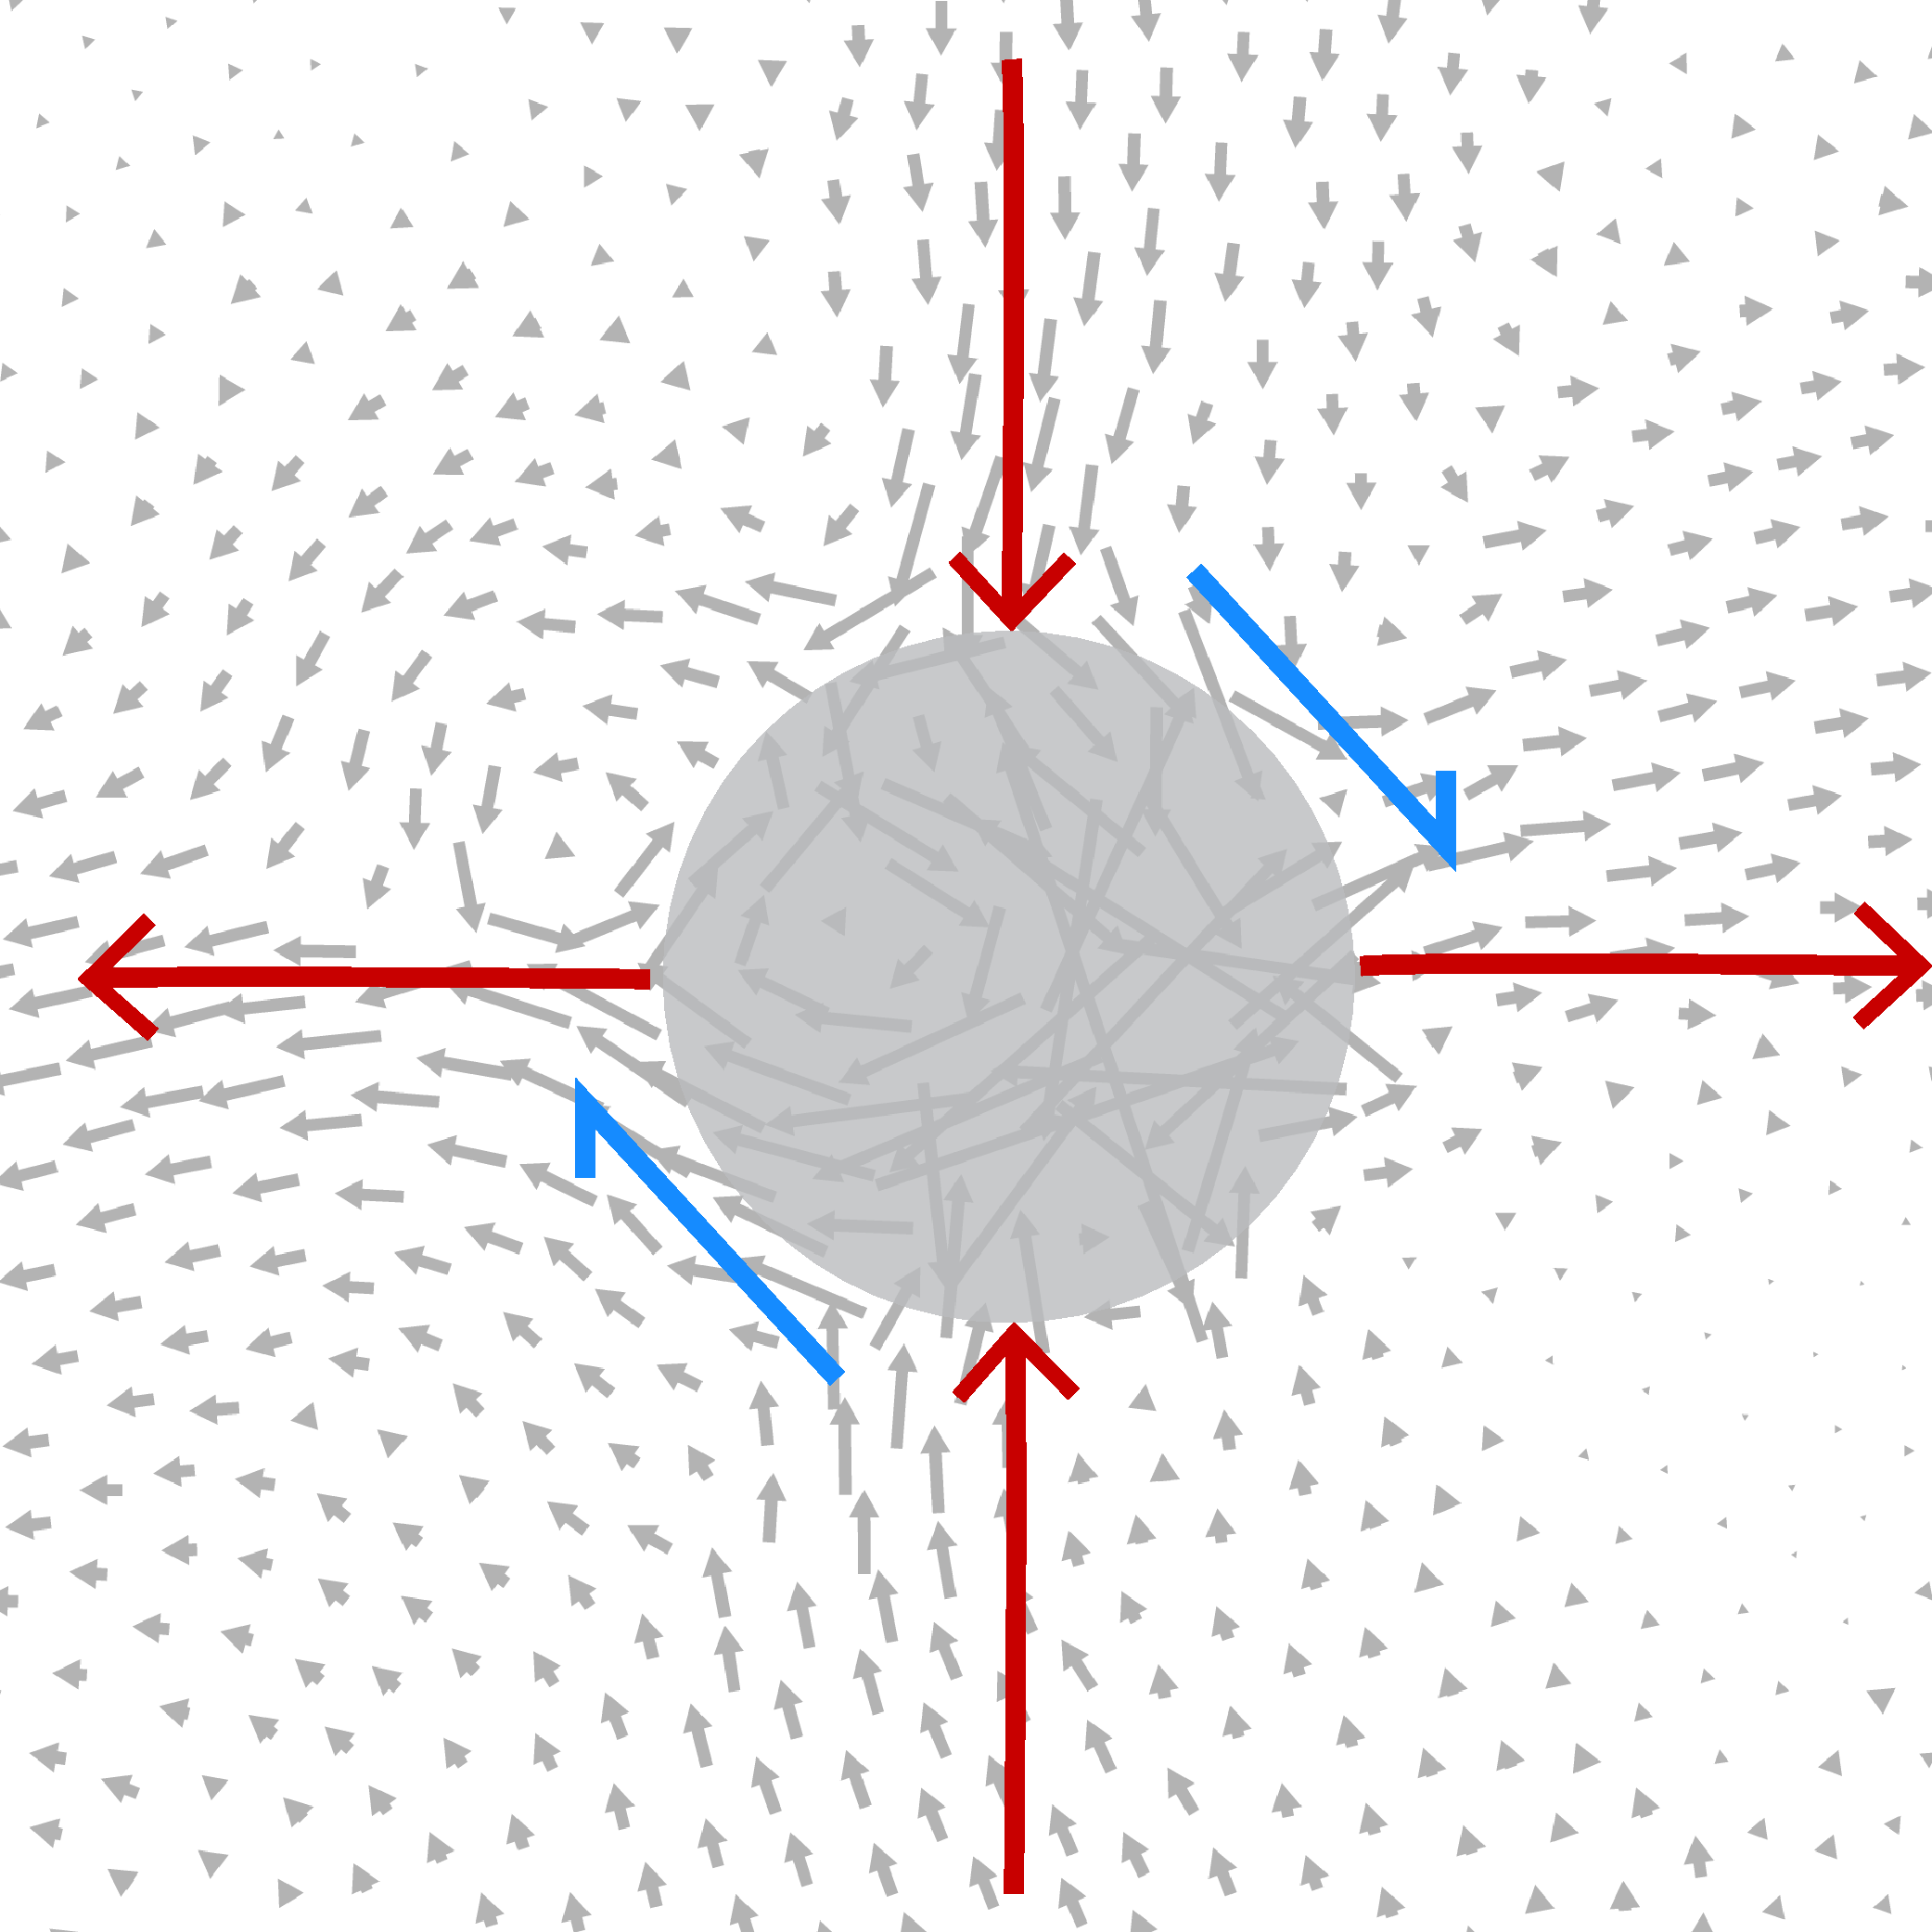
\includegraphics[width=0.85\linewidth]{1.b-exc_pureshear/zoomin-4.pdf}\caption{Alternatively, an excitation induces a simple shear in one side.}

% \onslide<10->\centering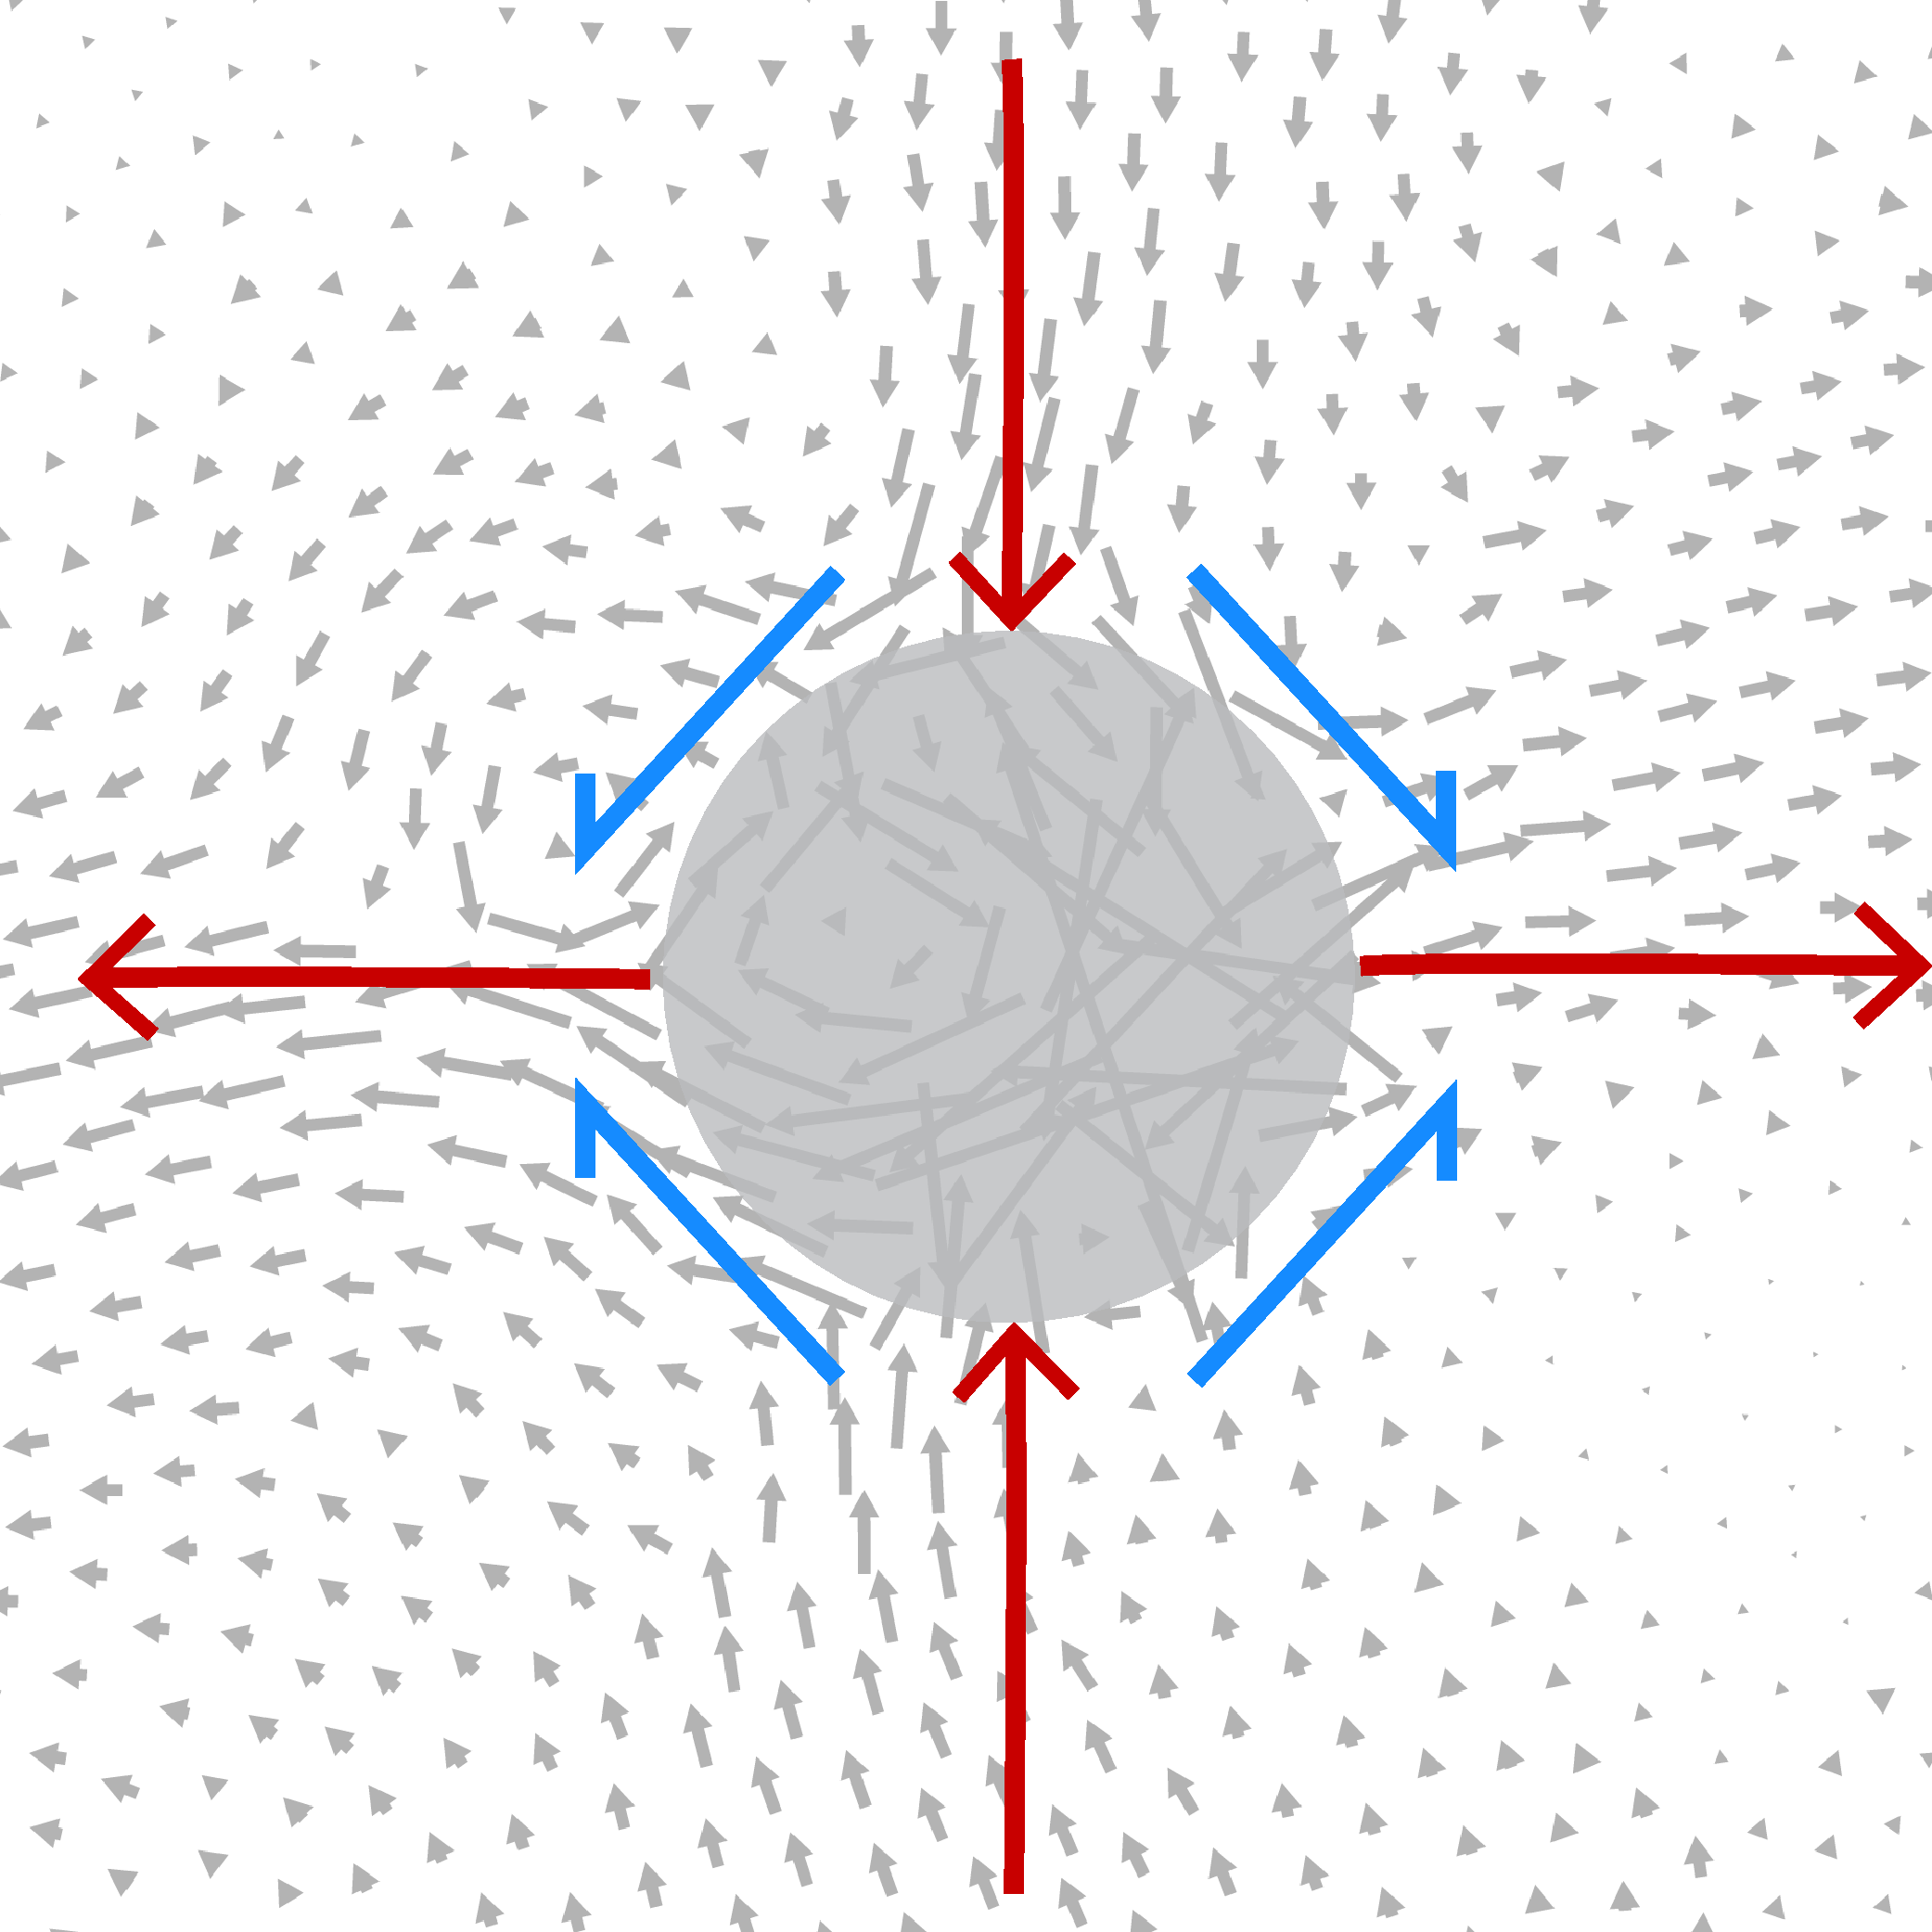
\includegraphics[width=0.85\linewidth]{1.b-exc_pureshear/zoomin-5.pdf}\caption{And induce an additional simple on the other side $\to$ \textbf{pure shear}.}
%\includegraphics[width=0.9\linewidth]{1.b-exc_pureshear/pureshear.jpg}

    
\end{overprint}
\end{figure}

\end{column}

\begin{column}[T]{0.6\textwidth}

\begin{enumerate}
\item<2-> Inherent states `=' amorphous solids %(for small deformations)

\item<13-> The linear theory of elasticity: %Energetic cost arises from the elastic reorganization of its surroundings:
\onslide<13->{
\begin{center}
\begin{minipage}{0.9\linewidth}

\begin{block}{\centering Excitation Energy Cost $J_\sigma$}

\begin{gather*}
\Delta F^\ddagger(T) = G^\mathrm{IS}(T) \left(\pi R_\mathrm{exc}^2 \right) \epsilon_c^2 \quad \text{(in 2D)}
\\
J_\sigma = \lim_{T \to 0} \Delta F^\ddagger(T)
%G^\mathrm{IS}(T) = \left\langle C_{xyxy}(\{ \* R^\alpha\})\right\rangle_\mathrm{IS}
\end{gather*}
\end{block}
\end{minipage}
\end{center}
}

\item<14-> Compute $G^\mathrm{IS}(T)$ from first-principles. (Lutsko, \textit{J. App. Phys.} (1989)).
\item<15-> Compute  $R_\mathrm{exc}$ and $\epsilon_\mathrm{c}$ from structural info, e.g., the radial distribution function. %(Hasyim, Mandadapu, \textit{J. Chem. Phys.} (2021)).
\end{enumerate}

\end{column}
\end{columns}

\end{frame}

